\documentclass[
	ngerman,
	ruledheaders=section,%Ebene bis zu der die Überschriften mit Linien abgetrennt werden, vgl. DEMO-TUDaPub
	class=report,% Basisdokumentenklasse. Wählt die Korrespondierende KOMA-Script Klasse
	thesis={type=master},% Dokumententyp Thesis
	accentcolor=2c, % Akzentfarbe FG rtm
	custommargins=false,
	marginpar=false,
	BCOR=10mm, % Bindekorrektur (etwas größere mittlere Ränder)
	parskip=half-, % Absatzkennzeichnung durch Abstand vgl. KOMA-Sript
	fontsize=11pt, % Basisschriftgröße laut Corporate Design ist mit 9pt häufig zu klein
  	twoside,
  	numbers=noendperiod,
  	fleqn,
  	captions=oneline, % Einzeilige Captions zentrieren
	captions=tableheading, % Für besseren Abstand bei TabellenÜBERschriften
  	IMRAD=false,
]{tudapub}


%%%%%%%%%%%%%%%%%%%
%Pakete einbinden
%%%%%%%%%%%%%%%%%%%
%%%%%%%%%%%%%%%%%%%
% Mathe-Umgebungen und Symbole
%%%%%%%%%%%%%%%%%%%
\usepackage{amsmath}
\usepackage{amssymb}

%%%%%%%%%%%%%%%%%%%
% TikZ für Blockschaltbilder und Skizzen
%%%%%%%%%%%%%%%%%%%
\usepackage{tikz}				% Zum Erzeugen von Bildern mit TikZ
% TikZstyles-Bibliothek f�r Blockschaltbilder

\usetikzlibrary{arrows}		
\usetikzlibrary{arrows.meta}
\usetikzlibrary{positioning}

\newcommand{\TikZscale}{1}
\newcommand{\mm}{*\TikZscale mm}
\tikzset{every picture/.style={node distance=4\mm, >=stealth'}}

%% Bl�cke
	% Rechteckige Bl�cke
	\tikzstyle{block}      = [draw, semithick, rectangle, minimum height=8\mm, minimum width=8\mm, inner sep=3pt]
	\tikzstyle{NLblock}    = [draw, semithick, rectangle, minimum height=8\mm, minimum width=8\mm, inner sep=3pt, double distance=1.2pt]
	\tikzstyle{PICblock}   = [draw, semithick, rectangle, minimum height=8\mm, minimum width=8\mm, inner sep=2pt]
	\tikzstyle{NLPICblock} = [draw, semithick, rectangle, minimum height=8\mm, minimum width=8\mm, inner sep=3pt, double distance=1.2pt]
	\tikzstyle{noblock}	   = [rectangle, inner sep=-0.6pt]

	% Dreieckige Bl�cke
	\tikzstyle{Rgain}			 = [draw, semithick, isosceles triangle, inner sep=1pt, minimum height=8\mm, isosceles triangle apex angle=60]
	\tikzstyle{Lgain}			 = [draw, semithick, isosceles triangle, inner sep=1pt, minimum height=8\mm, isosceles triangle apex angle=60, shape border rotate=180]
	\tikzstyle{Ugain}			 = [draw, semithick, isosceles triangle, inner sep=1pt, minimum height=8\mm, isosceles triangle apex angle=60, shape border rotate=90]
	\tikzstyle{Dgain}			 = [draw, semithick, isosceles triangle, inner sep=1pt, minimum height=8\mm, isosceles triangle apex angle=60, shape border rotate=-90]

	% Runde Bl�cke
	\tikzstyle{sum}   	   = [draw, semithick, circle, inner sep=1pt, minimum size=3\mm]
	\tikzstyle{branch}		 = [draw, circle, inner sep=0pt, minimum size=1\mm, fill=black]
	\tikzstyle{BRANCH}		 = [coordinate]


%% Verbindungselemente
	% Linien mit Pfeil
	\tikzstyle{to}  		= [->, thick]
	\tikzstyle{toNL}		= [->, thick, shorten >=0.9pt]
	\tikzstyle{NLto}		= [->, thick, shorten <=0.9pt]
	\tikzstyle{NLtoNL}	= [->, thick, shorten <=0.9pt, shorten >=0.9pt]
	
	\tikzstyle{TO}  		= [semithick, double distance=2pt, shorten >=2mm, decoration={markings,mark=at position 1 with {\arrow[semithick]{open triangle 60}}}, preaction={decorate},postaction={draw, line width=2pt, white, shorten >= 1.5mm}]
	
	\tikzstyle{TONL}  		= [semithick, double distance=2pt, shorten >=2.2mm, decoration={markings,mark=at position 1 with {\arrow[semithick]{open triangle 60}}, transform={xshift=-0.7pt}}, preaction={decorate},postaction={draw, line width=2pt, white, shorten >= 1.5mm}]
	
	\tikzstyle{NLTO}  		= [semithick, double distance=2pt, shorten <=0.9pt, shorten >=2mm, decoration={markings,mark=at position 1 with {\arrow[semithick]{open triangle 60}}}, preaction={decorate}, postaction={draw, line width=2pt, white, shorten >= 1.5mm}]
	
	\tikzstyle{NLTONL}  		= [semithick, double distance=2pt, shorten <=0.9pt, shorten >=2.2mm, decoration={markings,mark=at position 1 with {\arrow[semithick]{open triangle 60}}}, preaction={decorate},postaction={draw, line width=2pt, white, shorten >= 1.5mm}]
	
	\tikzstyle{innerWhite} = [semithick, white,line width=2pt, shorten >= 2mm, shorten <= 2mm]
	
	%\tikzstyle{TO}  		= [semithick, double distance=2pt, shorten >=2mm, decoration={markings,mark=at position 1 with {\arrow[semithick]{open triangle 60}}}, postaction={decorate}]
		%
	%\tikzstyle{TONL} = [semithick, double distance=2pt, shorten >=2.2mm, decoration={markings,mark=at position 1 with {\arrow[semithick]{open triangle 60}}, transform={xshift=-0.7pt}}, postaction={decorate}]
	%
	%\tikzstyle{NLTO} = [semithick, double distance=2pt, shorten <=0.79pt, shorten >=2mm, decoration={markings,mark=at position 1 with {\arrow[semithick]{open triangle 60}}}, postaction={decorate}]
	%
	%\tikzstyle{NLTONL} = [semithick, double distance=2pt, shorten <=0.79pt, shorten >=2.2mm, decoration={markings,mark=at position 1 with {\arrow[semithick]{open triangle 60}}, transform={xshift=-0.7pt}}, postaction={decorate}]
	

	% Linien ohne Pfeil 
	\tikzstyle{line}       = [thick]
	\tikzstyle{lineNL}     = [thick, shorten >= 0.6pt]
	\tikzstyle{NLline}     = [thick, shorten <= 0.6pt]
	\tikzstyle{NLlineNL}	 = [thick, shorten <= 0.6pt, shorten >= 0.6pt]
	
	% Doppellinien ohne Pfeil
	\tikzstyle{LINE}       = [semithick, double distance=2pt]
	\tikzstyle{LINENL}     = [semithick, double distance=2pt, shorten >= 0.9pt]
	\tikzstyle{NLLINE}     = [semithick, double distance=2pt, shorten <= 0.9pt]
	\tikzstyle{NLLINENL}	 = [semithick, double distance=2pt, shorten <= 0.9pt, shorten >= 0.9pt]
	
	\tikzstyle{neg}				 = [postaction={decorate,decoration={markings, mark=at position 1 with{\draw[-](-2pt,-3pt)--(-2pt,-7pt);}}}]
	
	\tikzstyle{labelabove} = [above, anchor=base, yshift=0.75ex]
	\tikzstyle{labelbelow} = [below, anchor=base, yshift=-2ex]
	\tikzstyle{labelright} = [right]
	\tikzstyle{labelleft}  = [left]
	
	
	% Pins und Labels
	\tikzstyle{every pin edge}	= [<-, thick]
	\tikzstyle{every pin}	 			= [pin distance=5\mm]
	\tikzstyle{every label}			= [font=\small]
	\tikzstyle{terminal}				= [coordinate]
	
	% extra Symbole f�r circuits-Library
	\tikzstyle{jack}	= [draw, circle, minimum size=1.5mm, inner sep=0]
 % rtm-eigene Bibliothek für Blockschaltbilder

%%%%%%%%%%%%%%%%%%%
% Plotten direkt in LaTeX
%%%%%%%%%%%%%%%%%%%
\usepackage{pgfplots}

%%%%%%%%%%%%%%%%%%%
% Bilder und Abbildungen
%%%%%%%%%%%%%%%%%%%
\usepackage{pdfpages}
\usepackage{graphicx}
\usepackage{caption}
\usepackage{subcaption}
\usepackage{float}
\usepackage{import}
\usepackage{color}
\usepackage{transparent}


%%%%%%%%%%%%%%%%%%%
%Sprachanpassung & Verbesserte Trennregeln
%%%%%%%%%%%%%%%%%%%
%\usepackage{acronym}
\usepackage[acronym]{glossaries}
\setacronymstyle{long-short}
%\usepackage{glossaries-extra}
\usepackage[english, main=ngerman]{babel}
\usepackage[autostyle]{csquotes}% Anführungszeichen vereinfacht
\usepackage{microtype}
\usepackage{etoolbox}


%%%%%%%%%%%%%%%%%%%
%Meine Makros einbinden
%%%%%%%%%%%%%%%%%%%
\newcommand{\eqp}{\ensuremath{\, \, \, .}}
\newcommand{\M}[1]{\textbf{#1}} %Matrix  M
\newcommand{\Mr}[1]{\textbf{#1}_\rho} %Matrix mit tiefgestelltem rho, M_rho
\newcommand{\Mtil}[1]{\tilde{\textbf{#1}}} %Matrix mit Tilde
\newcommand{\Mtilt}[2]{\tilde{\textbf{#1}}_{#2}} %Matrix mit Tilde mit tiefgestelltem arg2
\DeclareRobustCommand{\Mt}[2]{\textbf{#1}_{#2}} %Matrix M mit tiefgestelltem arg2


\DeclareRobustCommand{\w}[1]{\underline{#1}} %Vektor arg1 unterstrichen 
\DeclareRobustCommand{\wt}[2]{\underline{#1}_{#2}} %Vektor unterstrichen w mit tiefgestelltem arg2
\DeclareRobustCommand{\wr}[1]{\underline{#1}_{\rho}} %Vektor unterstrichen mit rho, w_rho

% Textbausteine
% =============
	% Produktnamen
	\newcommand*{\Matlab}{\textsc{Matlab}}
	\newcommand*{\Matlabreg}{\textsc{Matlab}\textsuperscript{\tiny \textregistered}}
	\newcommand*{\MatSim}{\textsc{Matlab/Simulink}}
	\newcommand*{\Simulink}{\textsc{Simulink}}
	\newcommand*{\Simulinkreg}{\textsc{Simulink}\textsuperscript{\tiny \textregistered}}

	% Das Makro |\name|\marg{person} formatiert einen Personennamen bspw. eines Erfinders oder Entdeckers gemäß |\name{Euler}| \arrow\ \name{Euler}.
	\newcommand*{\name}[1]{\textsc{#1}}
	\newcommand*{\GenderPl}[1]{{#1}\_innen}
	\newcommand*{\GendeSin}[1]{{#1}\_in}
% Makros für Einheiten, Exponenten
% ================================

	\newcommand*{\unit}[1]{\ensuremath{\mathrm{#1}}}
	
	% Wert mit Einheit (mit kleinem Leerzeichen dazwischen), aus Text- UND Math-Modus
	\newcommand*{\valunit}[2]{\ensuremath{#1\,\mrm{#2}}}
	
	
	% "°C", im Text- oder Mathe-Modus
	\newcommand*{\degC}{
		\ifmmode
		^\circ \mrm{C}%
		\else
		\textdegree C%
		\fi}
	
	\newcommand*{\degree}{
		\ifmmode
		^\circ%
		\else
		\textdegree%
		\fi}
	
	% Für Exponentenschreibweise ( Anwendung: 123\E{3} )
	\newcommand*{\E}[1]{\ensuremath{\cdot 10^{#1}}}
	
	\newcommand*{\eexp}[1]{\ensuremath{\mathrm{e}^{#1}}}
	\newcommand*{\iu}{\ensuremath{\mathrm{j}}}
	
	\newcommand*{\todots}{\ensuremath{,\,\hdots,\,}}

% Makros für Formeln
% ==================

	% Definition für Vektor und Matizen
	\newcommand*{\mat}[1]{{\ensuremath{\boldsymbol{\mathrm{#1}}}}}
	\newcommand*{\ma}[1]{{\ensuremath{\boldsymbol{\mathrm{#1}}}}}
	\newcommand*{\mas}[1]{\ensuremath{\boldsymbol{#1}}}
	\newcommand*{\ve}[1]{\ensuremath{\boldsymbol{#1}}}
	\newcommand*{\ves}[1]{\ensuremath{\boldsymbol{\mathrm{#1}}}}
	
	\newcommand*{\AP}{\ensuremath{\mathrm{AP}}}
	\newcommand*{\doti}{\ensuremath{(i)^\cdot}}
	
	\newcommand*{\inprod}[2]{\ensuremath{\langle #1,\,#2 \rangle}}
	
	\newcommand*{\ul}[1]{\underline{#1}}
	
	% gerades "d" (z.B. für Integral)
	\newcommand*{\ud}{\ensuremath{\mathrm{d}}}
	
	% normaler Text in Formeln
	\newcommand*{\tn}[1]{\textnormal{#1}}
	
	% nicht-kursive Schrift in Formeln
	\newcommand*{\mrm}[1]{\ensuremath{\mathrm{#1}}}
	
	% gerades "T" für Transponiert
	\newcommand*{\transp}{\ensuremath{\mathrm{T}}}
	
	% gerades "rg"
	\newcommand*{\rang}{\ensuremath{\operatorname{rg}}}
	
	% Für geklammerte Ausdrücke mit Index (Subscript)
	% (einmal mit kursiven Index, einmal mit geradem Index)
	\newcommand*{\grpsb}[2]{\ensuremath{\left(#1\right)_{#2}}}
	\newcommand*{\grprsb}[2]{\ensuremath{\left(#1\right)_{\mathrm{#2}}}}
	
	% Ableitungen und Integrale
		% "normale" Ableitung (mit geraden "d"s)
		\newcommand*{\normd}[2]{\ensuremath{\frac{\mathrm{d}#1}{\mathrm{d}#2}}}
		\newcommand*{\normdat}[3]{\ensuremath{\left.\frac{\mathrm{d} #1}{\mathrm{d} #2}\right|_{#3}}}
		
		% Materielle Ableitung
		\newcommand*{\matd}[2]{\ensuremath{\frac{\mathrm{D} #1}{\mathrm{D} #2}}}
		\newcommand*{\matdat}[3]{\ensuremath{\left.\frac{\mathrm{D} #1}{\mathrm{D} #2}\right|_{#3}}}
		
		% Partielle Ableitung
		\newcommand*{\partiald}[2]{\ensuremath{\frac{\partial #1}{\partial #2}}}
		\newcommand*{\partialdat}[3]{\ensuremath{\left.\frac{\partial #1}{\partial #2}\right|_{#3}}}
	
	
	% Transformationen
	\newcommand*{\FT}[1]{\ensuremath{\mathfrak{F}\left\{#1\right\}}}
	\newcommand*{\FTabs}[1]{\ensuremath{\left|\mathfrak{F}\left\{#1\right\}\right|}}
	\newcommand*{\IFT}[1]{\ensuremath{\mathfrak{F}^{-1}\left\{#1\right\}}}
	\newcommand*{\DFT}[1]{\ensuremath{\mathrm{DFT}\left\{#1\right\}}}
	\newcommand*{\DFTabs}[1]{\ensuremath{\left|\mathrm{DFT}\left\{#1\right\}\right|}}
	\newcommand*{\Laplace}[1]{\ensuremath{\mathfrak{L}\left(#1\right)}}
	\newcommand*{\InvLaplace}[1]{\ensuremath{\mathfrak{L^{-1}}\left(#1\right)}}
	\newcommand*{\invtrans}{\ensuremath{\quad\bullet\!\!-\!\!\!-\!\!\circ\quad}}
	\newcommand*{\trans}{\ensuremath{\quad\circ\!\!-\!\!\!-\!\!\bullet\quad}}
	
	
	\newcommand*{\mlfct}[1]{\texttt{#1}}
	\newcommand*{\mlvar}[1]{\texttt{#1}}
	
	
	% Manche textcomp-Zeichen funktionieren mit dem TU-Design nicht, diese können dann mit diesem
	% Befehl gesetzt werden.
	\newcommand*{\textcompstdfont}[1]{{\fontfamily{cmr} \fontseries{m} \fontshape{n} \selectfont #1}}

% Makros für Variablen
% ================================
\newcommand*{\amax}{\ensuremath{a_{\textrm{max}}}}
\newcommand*{\amin}{\ensuremath{a_{\textrm{min}}}}
\newcommand*{\jmax}{\ensuremath{j_{\textrm{max}}}}
\newcommand*{\jmin}{\ensuremath{j_{\textrm{min}}}}
\newcommand*{\opt}[1]{\ensuremath{{#1}^*}}
\newcommand*{\fofx}{\ensuremath{f(\ve{x})}}
\newcommand*{\J}{\ensuremath{J(\ve{x}(t),\ve{u}(t),t)}}
\newcommand*{\Vofxoftf}{\ensuremath{V(\ve{x}(t_f),t_f)}}
\newcommand*{\Vofxoftone}{\ensuremath{\tilde{V}(\ve{x}(t_1),t_1)}}
\newcommand*{\Vofxoftfallgemein}{\ensuremath{\bar{V}(\ve{x}(t_f),t_f)}}
\newcommand*{\Vofxoftoftonefallgemein}{\ensuremath{\hat{V}(\ve{x}(t_f),\ve{x}(t_1),t_f,t_1)}}
\newcommand*{\variation}[1]{\ensuremath{\ve{\delta}_{#1}}}
\newcommand*{\dtint}[1]{\ensuremath{\textrm{d}{#1}}}
% Makros für x(t) Variablen
% ================================
\newcommand*{\xzero}{\ensuremath{\ve{x}_0}}
\newcommand*{\xoft}{\ensuremath{\ve{x}(t)}}
\newcommand*{\xoftf}{\ensuremath{\ve{x}(t_f)}}
\newcommand*{\xoftzero}{\ensuremath{\ve{x}(t_0)}}
\newcommand*{\xoftone}{\ensuremath{\ve{x}(t_1)}}
\newcommand*{\xofti}{\ensuremath{\ve{x}(t_i)}}
\newcommand*{\xoftoneminus}{\ensuremath{\ve{x}(t_1^-)}}
\newcommand*{\xoftoneplus}{\ensuremath{\ve{x}(t_1^+)}}
\newcommand*{\xoptoft}{\ensuremath{\opt{\ve{x}}(t)}}
\newcommand*{\xoptoftf}{\ensuremath{\opt{\ve{x}}(t_f)}}
\newcommand*{\xoptoftzero}{\ensuremath{\opt{\ve{x}}(t_0)}}
\newcommand*{\xoptoftfopt}{\ensuremath{\opt{\ve{x}}(\opt{t_f})}}
% Makros für x(tau) Variablen
% ================================
\newcommand*{\xoftau}{\ensuremath{\ve{x}(\tau)}}
\newcommand*{\xoftauf}{\ensuremath{\ve{x}(\tau_f)}}
\newcommand*{\xoftauzero}{\ensuremath{\ve{x}(\tau_0)}}
\newcommand*{\xoptoftau}{\ensuremath{\opt{\ve{x}}(t\tau)}}
\newcommand*{\xoptoftauf}{\ensuremath{\opt{\ve{x}}(\tau_f)}}
\newcommand*{\xoptoftauzero}{\ensuremath{\opt{\ve{x}}(\tau_0)}}
\newcommand*{\xoptoftaufopt}{\ensuremath{\opt{\ve{x}}(\opt{\tau_f})}}
% Makros für dx(t) Variablen
% ================================
\newcommand*{\dx}{\ensuremath{\dot{\ve{x}}}}
\newcommand*{\dxoft}{\ensuremath{\dot{\ve{x}}(t)}}
\newcommand*{\dxoftf}{\ensuremath{\dot{\ve{x}}(t_f)}}
\newcommand*{\dxoftzero}{\ensuremath{\dot{\ve{x}}(t_0)}}
\newcommand*{\dxoptoft}{\ensuremath{\dot{\ve{x}}^*(t)}}
\newcommand*{\dxoptoftf}{\ensuremath{\dot{\ve{x}}^*(t_f)}}
\newcommand*{\dxoptoftfopt}{\ensuremath{\dot{\ve{x}}^*(\opt{t_f})}}
% Makros für dx(tau) Variablen
% ================================
\newcommand*{\dxoftau}{\ensuremath{\ve{x}'(\tau)}}
\newcommand*{\dxoftauf}{\ensuremath{\ve{x}'(\tau_f)}}
\newcommand*{\dxoftauzero}{\ensuremath{\ve{x}'(\tau_0)}}
\newcommand*{\dxoptoftau}{\ensuremath{\ve{x}'^*(\tau)}}
\newcommand*{\dxoptoftauf}{\ensuremath{\ve{x}'^*(\tau_f)}}
\newcommand*{\dxoptoftaufopt}{\ensuremath{\ve{x}'^*(\opt{\tau_f})}}
% Makros für u(t) Variablen
% ================================
\newcommand*{\uoft}{\ensuremath{\ve{u}(t)}}
\newcommand*{\uoftf}{\ensuremath{\ve{u}(t_f)}}
\newcommand*{\uoftzero}{\ensuremath{\ve{u}(t_0)}}
\newcommand*{\uoptoft}{\ensuremath{\opt{\ve{u}}(t)}}
\newcommand*{\uoptoftf}{\ensuremath{\opt{\ve{u}}(t_f)}}
\newcommand*{\uoptoftfopt}{\ensuremath{\opt{\ve{u}}(\opt{t_f})}}
% Makros für u(tau) Variablen
% ================================
\newcommand*{\uoftau}{\ensuremath{\ve{u}(\tau)}}
\newcommand*{\uoftauf}{\ensuremath{\ve{u}(\tau_f)}}
\newcommand*{\uoftauzero}{\ensuremath{\ve{u}(\tau_0)}}
\newcommand*{\uoptoftau}{\ensuremath{\opt{\ve{u}}(\tau)}}
\newcommand*{\uoptoftauf}{\ensuremath{\opt{\ve{u}}(\tau_f)}}
\newcommand*{\uoptoftaufopt}{\ensuremath{\opt{\ve{u}}(\opt{\tau_f})}}
% Makros für lambda(t) Variablen
% ================================
\newcommand*{\lambdaoft}{\ensuremath{\ve{\lambda}(t)}}
\newcommand*{\lambdaoftf}{\ensuremath{\ve{\lambda}(t_f)}}
\newcommand*{\lambdaoftone}{\ensuremath{\ve{\lambda}(t_1)}}
\newcommand*{\lambdaoftzero}{\ensuremath{\ve{\lambda}(t_0)}}
\newcommand*{\lambdaoftoneminus}{\ensuremath{\ve{\lambda}(t_1^-)}}
\newcommand*{\lambdaoftoneplus}{\ensuremath{\ve{\lambda}(t_1^+)}}
% Makros für lambda(tau) Variablen
% ================================
\newcommand*{\lambdaoftau}{\ensuremath{\ve{\lambda}(\tau)}}
\newcommand*{\lambdaoftauf}{\ensuremath{\ve{\lambda}(\tau_f)}}
% Makros für dlambda(t) Variablen
% ================================
\newcommand*{\dlambda}{\ensuremath{\dot{\ve{\lambda}}}}
\newcommand*{\dlambdaoft}{\ensuremath{\dot{\ve{\lambda}}(t)}}
% Makros für dlambda(tau) Variablen
% ================================
\newcommand*{\dlambdaoftau}{\ensuremath{\ve{\lambda}'(\tau)}}
% Makros für z(t) Variablen
% ================================
\newcommand*{\zzero}{\ensuremath{\ve{z}_0}}
\newcommand*{\zoft}{\ensuremath{\ve{z}(t)}}
\newcommand*{\zoftf}{\ensuremath{\ve{z}(t_f)}}
\newcommand*{\zoftzero}{\ensuremath{\ve{z}(t_0)}}
\newcommand*{\zoptoft}{\ensuremath{\opt{\ve{z}}(t)}}
\newcommand*{\zoptoftf}{\ensuremath{\opt{\ve{z}}(t_f)}}
\newcommand*{\zoptoftzero}{\ensuremath{\opt{\ve{z}}(t_0)}}
\newcommand*{\zoptoftfopt}{\ensuremath{\opt{\ve{z}}(\opt{t_f})}}
% Makros für z(tau) Variablen
% ================================
\newcommand*{\zoftau}{\ensuremath{\ve{z}(\tau)}}
\newcommand*{\zoftauf}{\ensuremath{\ve{z}(\tau_f)}}
\newcommand*{\zoftauzero}{\ensuremath{\ve{z}(\tau_0)}}
\newcommand*{\zoptoftau}{\ensuremath{\opt{\ve{z}}(\tau)}}
\newcommand*{\zoptoftauf}{\ensuremath{\opt{\ve{z}}(\tau_f)}}
\newcommand*{\zoptoftauzero}{\ensuremath{\opt{\ve{z}}(\tau_0)}}
\newcommand*{\zoptoftaufopt}{\ensuremath{\opt{\ve{z}}(\opt{\tau_f})}}
% Makros für dz(t) Variablen
% ================================
\newcommand*{\dz}{\ensuremath{\dot{\ve{z}}}}
\newcommand*{\dzoft}{\ensuremath{\dot{\ve{z}}(t)}}
\newcommand*{\dzoftf}{\ensuremath{\dot{\ve{z}}(t_f)}}
\newcommand*{\dzoftzero}{\ensuremath{\dot{\ve{z}}(t_0)}}
\newcommand*{\dzoptoft}{\ensuremath{\dot{\ve{z}}^*(t)}}
\newcommand*{\dzoptoftf}{\ensuremath{\dot{\ve{z}}^*(t_f)}}
\newcommand*{\dzoptoftfopt}{\ensuremath{\dot{\ve{z}}^*(\opt{t_f})}}
% Makros für dz(tau) Variablen
% ================================
\newcommand*{\dzoftau}{\ensuremath{\ve{z}'(\tau)}}
\newcommand*{\dzoftauf}{\ensuremath{\ve{z}'(\tau_f)}}
\newcommand*{\dzoftauzero}{\ensuremath{\ve{z}'(\tau_0)}}
\newcommand*{\dzoptoftau}{\ensuremath{\ve{z}'^*(\tau)}}
\newcommand*{\dzoptoftauf}{\ensuremath{\ve{z}'^*(\tau_f)}}
\newcommand*{\dzoptoftaufopt}{\ensuremath{\ve{z}'^*(\opt{\tau_f})}}
% Makros für Ttransformation Variablen
% ================================
\newcommand*{\Ttransoftau}{\ensuremath{\mathcal{T}(\tau)}}
\newcommand*{\Ttransoftauzero}{\ensuremath{\mathcal{T}(\tau_0)}}
\newcommand*{\Ttransoftauf}{\ensuremath{\mathcal{T}(\tau_f)}}
% Makros für dTtransformation Variablen
% ================================
\newcommand*{\dTtransoftau}{\ensuremath{\mathcal{T}'(\tau)}}
\newcommand*{\dTtransoftauzero}{\ensuremath{\mathcal{T}'(\tau_0)}}
\newcommand*{\dTtransoftauf}{\ensuremath{\mathcal{T}'(\tau_f)}}



%%%%%%%%%%%%%%%%%%%
%Literaturverzeichnis
%%%%%%%%%%%%%%%%%%%
\catcode30=12  % Workaround for current biblatex problem (https://tex.stackexchange.com/questions/564990/error-after-miktex-reinstall-text-line-contains-an-invalid-character)
\usepackage[backend=biber,style=ieee,bibencoding=utf8]{biblatex}
\addbibresource{./Bib/literature.bib}

% ======================================================
% Fix für Fehlermeldungen 'Undifined control sequence' und 'Missing number, treated as zero.' bei gestapelten Akzenten in der Mathe-Umgebung. (z.B. \dot{\hat{x}})
% Der Fehler tritt auf bei tuda-ci v3.10 (Feb. 2021) in Kombination mit dem amsmath package.
%
% BITTE PRÜFEN, OB DER FEHLER NOCH BESTEHT UND DEN WORKAROUND GGF. WIEDER ENTFERNEN
%
% workaround/solution by skillmon posted here
% https://tex.stackexchange.com/questions/482281/math-accent-symbol-over-parentheses-enclosing-accented-symbol-amsmath
\makeatletter
\protected\def\mathaccentV#1#2#3#4#5%
  {%
    \ifmmode
      \mathaccentV@do{#2}{#3}{#4}{#5}%
    \else
      \@xp\nonmatherr@\csname #1\endcsname
    \fi
  }
\def\mathaccentV@do#1#2#3#4%
  {%
    \global\let\macc@nucleus\@empty
    \mathaccent"\accentclass@#1#2#3{#4}\macc@nucleus
  }
\makeatother
% ======================================================

\makeglossaries


%\newacronym{FAS}{FAS}{Fahrerassistenzsysteme}
%\newacronym{ACC}{ACC}{Adaptive Cruise Control}
%\newacronym{FSRA}{FSRA}{Full Speed Range Adaptive Cruise Control}
%\newacronym{FSW}{FSW}{Fahrstreifenwechsel}
\newglossaryentry{FAS}{name=FAS,description={Fahrassistenzsystem}}
\newglossaryentry{ACC}{name=ACC,description={Adaptive Cruise Control}}
\newglossaryentry{FSRA}{name=FSRA,description={Full Speed Range Adaptive Cruise Control}}
\newglossaryentry{FSW}{name=FSW,description={Fahrstreifenwechsel}}
\newglossaryentry{LKS}{name=LKS,description={Lane Keeping Support}}

\begin{document}
% =================================================================================
% Header mit allen Metadaten etc. 
% =================================================================================
\Metadata{	% Metadaten im erzeugten PDF/A
	title=Masterthesis Markus Amann,
	author=Markus Amann,
	keywords={TU Darmstadt \sep Corporate Design \sep LaTeX},
}

\title{Trajektorienplanung als dynamisches Optimalsteuerungsproblem und Interpretation des Lösungsraums für Fahrkomfort im automatisierten Fahren}
\subtitle{\textmd{Studiengang Elektrotechnik und Informationstechnik}}
\author[Markus Amann]{Markus Amann}
\reviewer*[Erstprüfer,Betreuer]{Prof. Dr.-Ing. Ulrich Konigorski \and Wi Mi M.Sc. Alexander Steinke} % erst ab Version v3.06 (2020-10-20) des tuda-ci-Pakets möglich

\department{etit}

\addTitleBox{
\includegraphics[width=\linewidth]{Bilder/rtm_mit_schrift}}

%\date{\today}
\submissiondate{4. Juli 2022}

\lowertitleback{
	Technische Universität Darmstadt\\
	Institut für Automatisierungstechnik und Mechatronik\\
	Fachgebiet Regelungstechnik und Mechatronik\\
	Prof. Dr.-Ing. Ulrich Konigorski\\
}

\frontmatter
\maketitle

\clearpage
\setcounter{page}{1}
\section*{Aufgabenstellung}

%\documentclass[
%	paper=a4,
%	ngerman,
%	accentcolor=2c, % Akzentfarbe FG rtm
%	type=announcement,
%	marginpar=false,
%	fleqn,
%	class=report,
%	fontsize=11pt
%	]{tudaposter}
%
%%%%%%%%%%%%%%%%%%%%
%%Sprachanpassung & Verbesserte Trennregeln
%%%%%%%%%%%%%%%%%%%%
%\usepackage[english, main=ngerman]{babel}
%\usepackage[autostyle]{csquotes}% Anführungszeichen vereinfacht
%\usepackage{microtype}
%
%\usepackage{amsmath,amssymb}
%
%\usepackage{url}
%
%%%%%%%%%%%%%%%%%%%%
%%Literaturverzeichnis
%%%%%%%%%%%%%%%%%%%%
%\catcode30=12  % Workaround for current biblatex problem (https://tex.stackexchange.com/questions/564990/error-after-miktex-reinstall-text-line-contains-an-invalid-character)
%\usepackage[backend=biber,style=ieee,bibencoding=utf8]{biblatex}
%%\addbibresource{model_fidelity.bib}
%
%\renewcommand*{\bibfont}{\small}
%\newcommand{\un}[1]{\, \text{#1}}
%\newcommand{\ve}[1]{\mathbf{#1}}
%\newcommand{\veG}[1]{\text{\boldmath{$#1$}}}
%
%\begin{document}
%
%\title{Trajektorienplanung als dynamisches Optimalsteuerungsproblem und Interpretation des Lösungsraums für Fahrkomfort im automatisierten Fahren \vspace{0.2cm}}
%\subtitle{Aufgabenstellung zur Masterthesis}
%\titleinfo{Betreuer: Alexander Steinke, M.Sc.\\ \today}
%\addTitleBox{
\includegraphics[width=\linewidth]{rtm_mit_schrift}}
%
%\maketitle
%%\section*{Aufgabenbeschreibung}
%
%%Zum numerischen Lösen Dynamischer Optimierungsprobleme können direkte und indirekt
%
%%Ein häufiger Ansatz zum Lösen dynamische Optimierungsprobleme ist die 
%
%%Dynamische Optimierungsprobleme lassen sich analytisch (Dynamische Optimierung) oder numerisch (Statische Optimierung) lösen. Während in der statischen Optimierung

Die allgemeine Struktur eines Optimalsteuerungsproblems lautet
%
\begin{equation*} \begin{aligned}
		\min\limits_{\ve{u}(t)} \ \ \ & J(\ve{u})=V(\ve{x}(t_\text{f}),t_\text{f}) + \int_{t_0}^{t_\text{f}}l(\ve{x}(t),\ve{u}(t),t)\text{d}t \\
		\text{u.B.v.} \ \ \ & \dot{\ve{x}}(t)=\ve{f}(\ve{x}(t),\ve{u}(t),t), \ \ve{x}(t_0)=\ve{x}_0\\ 
		& \mathbf{g}(\ve{x}(t_\text{f}),t_\text{f}) = \ve{0} \\
		& \mathbf{h}(\ve{x}(t),\ve{u}(t),t) \leq \ve{0}.
\end{aligned} \end{equation*}
%
Häufig werden dynamische Optimierungsprobleme (OP) mithilfe direkter Verfahren numerisch gelöst. 
In diesem Fall wird das dynamische in ein statisches OP überführt und der endliche Lösungsvektor $\ve{u}_\text{opt} \in \mathcal{U} \subseteq \mathbb{R}^m$ berechnet. 
Direkte Verfahren haben den Vorteil, dass Zustandsbeschränkungen leichter berücksichtigt werden können und der Konvergenzbereich größer ist. 
Indirekte Verfahren hingegen liefern eine Einsicht in die Struktur der optimalen Lösung.

In der dynamischen Optimierung hingegen werden Funktionen $\ve{u}(t)$ einer unabhängigen Variable $t$ gesucht. 
Mithilfe der Variationsrechnung können Optimalitätsbedingungen hergeleitet werden, die ein Randwertproblem formulieren. 
Die Lösung dieses Randwertproblems liefert in der Folge die optimale Steuertrajektorie $\ve{u}_\text{opt}(t)$. 
Jedoch ist das Lösen des Randwertproblems für nichtlineare Systeme häufig schwierig, weswegen auf numerische Verfahren zurückgegriffen werden muss.

Um im automatisierten Fahren (AD) gezielt Fahrprofile mittels einer optimalen Trajektorienplanung erstellen zu können, ist ein tieferes Verständnis der optimalen Lösung erforderlich. 
Mit einem direkten Verfahren ist die Interpretation der Lösung schwierig, da die Lösung aus reinen Zahlenwerten besteht. 
Zwar könnte ein gewünschtes Fahrverhalten in definierten Fahraufgaben durch zusätzliche Terme im Gütemaß und Anpassung der Gewichte erzielt werden, jedoch ist eine Übertragung auf andere Fahraufgaben fraglich. 
Eine parametrierte Steuertrajektorie $\ve{u}_\text{opt}(t)$ würde die Interpretation erheblich vereinfachen.


Ziele dieser Arbeit sind folgende Punkte:
\begin{enumerate}
	\item Übersicht für Lösungsverfahren dynamischer OPs und Einordnung des AD-Planungsproblems
	\item Erstellen von dynamischen OPs, die durch Variationsrechnung lösbar sind und Lösen dieser
	\begin{enumerate}
		\item Geeignete Fahrszenarien (z.B. Geradeausfahrt, Kurve, Geraden-Kurven-Kombination, Spurwechsel)
		\item Geeignete Komfortmerkmale (z.B. Beschleunigung, Ruck, Fahrdauer)
		\item Berücksichtigung von Begrenzungen
	\end{enumerate}
	\item Interpretation der Lösungenstrajektorien hinsichtlich des dargestellten Funktionenraums 
	\item Einordnung im Kontext Fahrkomfort
\end{enumerate}

Die Ergebnisse sind geeignet zu visualisieren und zu dokumentieren. Die aktuelle Fassung der Richtlinien zur Anfertigung von Abschlussarbeiten ist zu beachten.


%%Technische Universität Darmstadt \\
%%Institut für Automatisierungstechnik und Mechatronik \\
%%Fachgebiet Regelungstechnik und Mechatronik \\
%%Prof. Dr.-Ing. Ulrich Konigorski
%
%%\vspace*{\fill} {\tiny
%%\printbibliography[heading=none]}
%
%\end{document}


\vspace{0.5cm}
\begin{tabular}{ll}
	Beginn: 	& ------ \\
	Ende: 		& ------ \\
	Seminar: 	& ------ \\
\end{tabular}
\clearpage

\affidavit

\section*{Kurzfassung}
Zusammenfassung entsprechend der Dokumentensprache. In diesem Fall Deutsch.
\section*{Abstract}
Additional abstract in English.	

\cleardoublepage

\tableofcontents
\cleardoublepage

\mainmatter


% =================================================================================
% Kapitel und Sections etc.
% =================================================================================
\chapter{Einleitung}\label{cha:Einleitung}

- kurze erklärung was fahrfremde Tätigkeit bedeutet und welche relevanz das für autonomes Fahren hat. 
- kurz ein paar Worte zu Kinetose und Hinweis darauf, dass es später noch genauer erklärt wird
\glsadd{utc}
\chapter{Fahrkomfort und Einordnung in den Kontext Automatisiertes Fahren}\label{cha:Komfort}
In diesem Kapitel soll der Begriff \glqq Fahrkomfort\grqq~in den Kontext \gls{AD} eingeordnet werden. Dazu wird zunächst die Bedeutung des Begriffs genauer betrachtet und die Verbindung zwischen Fahrkomfort und Sicherheitsempfinden dargelegt. Anschließend werden verschiedene Einflussfaktoren auf die Komfortwahrnehmung während des Fahrens thematisiert. Dabei wird das Phänomen der Kinetose genauer erklärt und speziell auf dessen Bedeutsamkeit für die Entwicklung automatisierter Fahrzeuge eingegangen. Abschließend werden mithilfe von Literaturwerten Grenzwerte für die als relevant erachteten Einflüsse untersucht. 
%\section{Begriffsdefinition Komfort}
%Während der Begriff ``Komfort'' im alltäglichen Sprachgebrauch eine sehr vielseitige Bedeutung hat und dabei sowohl zur Beschreibung positiver Empfindungen wie Wohlbehagen und Zufriedenheit, als auch in negierter Form zur Beschreibung negativer Gefühle wie Unwohlsein und Unzufriedenheit verwendet wird, wird bei der wissenschaftlichen Verwendung oftmals stärker differenziert. Es exisitieren verschiedene Modelle, die alle darauf abzielen, eine allgemeine Definition von Komfort zu liefern. Im Sinne der besseren Unterscheidbarkeit und damit einer genaueren Anwendung der entsprechenden Bedeutung, wird häufig zusätzlich der Begriff ``Diskomfort'' verwendet. In \cite{Zhang} wurden in einer Studie Faktoren für das Empfinden von Komfort und Diskomfort beim Sitzen identifiziert, wodurch sich die beiden Begriffe differenzierter verwenden lassen. Während Komfort durch Gefühle, die allgemein als positiv wahrgenommen werden, wie Entspanntheit, Ruhe und Zufriedenheit, klassifiziert wird, zeichnet sich Diskomfort vor allem durch negativ konnotierte Empfindungen, wie Müdigkeit und Rastlosigkeit, aber auch durch biometrische Faktoren, die spürbare Schmerzen verursachen, aus. Die Autoren leiten ein Modell her, in dem Komfort und Diskomfort zwei orthogonale Größen sind, die auch gleichzeitig erfahrbar sind. Während die Abwesenheit von Diskomfort nicht automatisch zur Zunahme von Komfort führt (dasselbe gilt auch anders herum), führt eine Zunahme von Diskomfort zwangsläufig zu einer Abnahme von Komfort. Wie Festner in \cite{Festner_diss} herausarbeitet, ist die Beseitigung von Diskomfort eine notwendige, jedoch nicht hinreichende Bedingung für das Empfinden von Komfort. Da jedoch unangenehme Situationen oftmals deutlicher explizit als solche wahrgenommen werden können, denn angenehme Situationen als angenehm, kann auch der erlebte Diskomfort als Kriterium für den fehlenden Komfort genutzt werden \cite{Festner}. 
%
%Ein weiteres Modell, welches breite Verwendung findet, ist die Komfortpyramide nach Krist \cite{Krist}. 
%\begin{figure}[h]
%	\centering
%	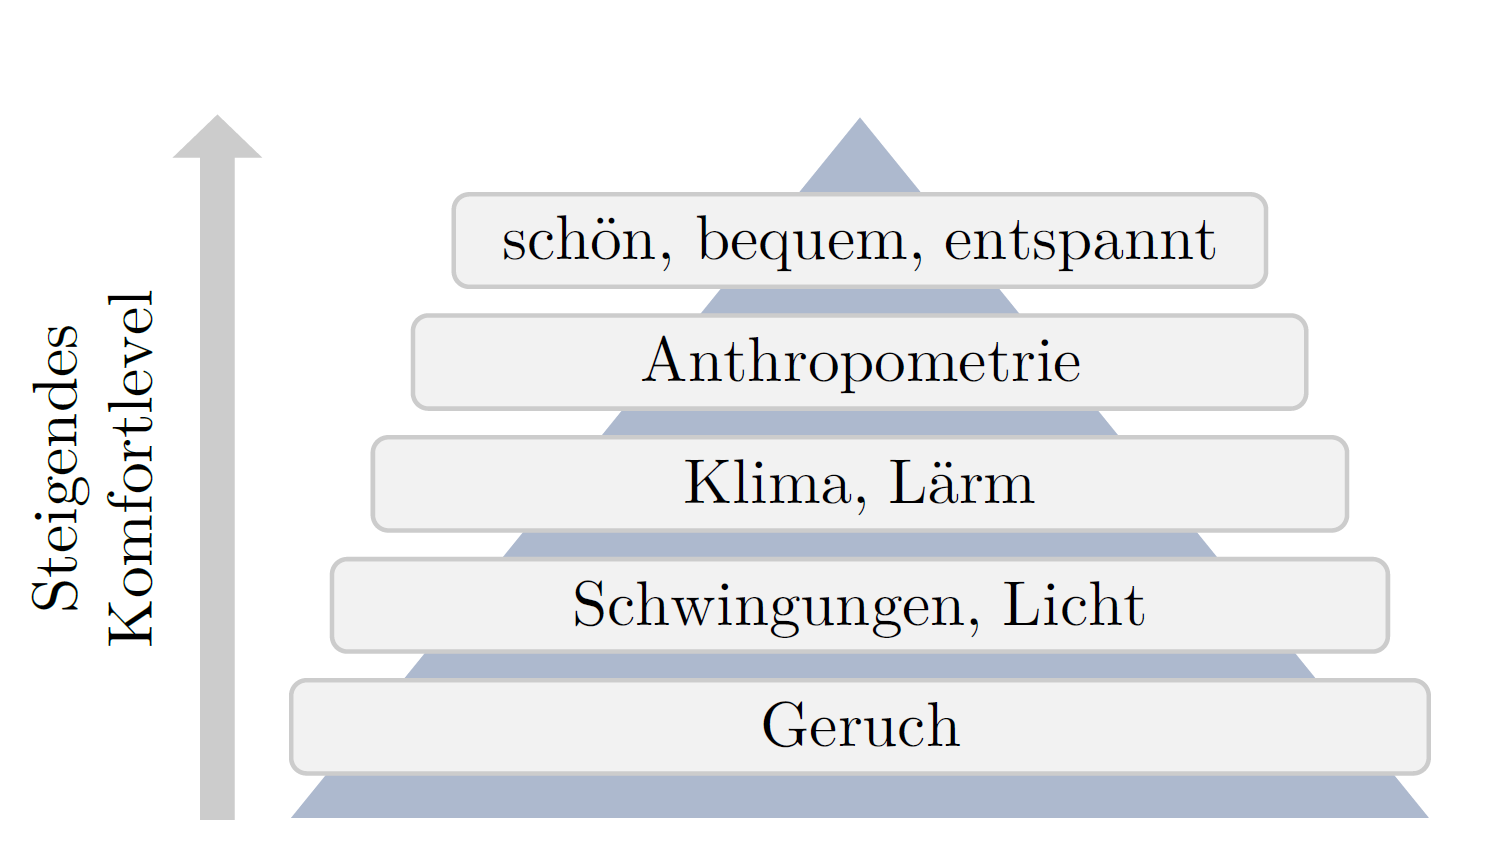
\includegraphics[scale=0.3]{./Bilder/komfortpyramide.png}
%	\label{fig:komfortpyramide}
%	\caption{Komfortpyramide aus \cite{Festner}, zitiert nach \cite{Krist}}
%\end{figure}
%
%In dieser Pyramide nimmt das Komfortlevel, ausgehend von sehr elementaren Faktoren wie Geruch und Lichteinflüssen, stetig zu. Um ein hohes Maß an Komfort zu erzielen, müssen notwendiger Weise zunächst die unteren, grundlegenden Bedingungen erfüllt sein. Zwar werden in diesem Modell Komfort und Diskomfort nicht so streng von einander getrennt, wie in \cite{Zhang}, allerdings ist die Bedingung, dass die Faktoren auf den unteren Ebenen zuerst erfüllt sein müssen damit auch auf den oberen Ebenen die Komfortbedingungen erfüllt werden können, vergleichbar mit der notwendigen Beseitigung von Diskomfort. Neben der qualitativen Beschreibung von Komfort, die alle Modelle gemein haben, unterscheiden sich die Ergebnisse, die unter Verwendung dieser Modelle erzielt werden, dennoch zum Teil stark, da die Komfortwahrnehmung sehr subjektiv ist und sich zwischen einzelnen Personen stark unterscheiden kann. Es lassen sich zwar einzelne Merkmale als komfortabel oder unkomfortabel klassifizieren, allerdings geht aus den Modellen nicht eindeutig hervor, wie stark die einzelnen Merkmale das persönliche Komfortempfinden beeinflussen. Zum Beispiel entwickelt jeder Mensch seine eigene Komfortpyramide, abhängig von ganz persönlichen Faktoren und Erfahrungen \cite{Krist}.
 
\section{Fahrkomfort im Kontext Automatisiertes Fahren}\label{sec:fahrkomfort}
Mit zunehmender Automatisierung von Fahraufgaben rückt auch der Fahrkomfort immer mehr in den Fokus. Es ist nicht davon auszugehen, dass hochautomatisierte oder autonome Fahrzeuge, deren Fahrweise von \GenderPl{Passagier} als unkomfortabel empfunden wird, eine hohe Akzeptanz finden werden. Damit sich überhaupt ein komfortables Gefühl während einer automatisierten Fahrt einstellen kann, muss bei den fahrzeugführenden Personen ein Gefühl von Sicherheit herrschen \cite{Festner.2019}. Nicht nur für unbeteiligte Dritte wie \GenderPl{Fußgänger} oder andere \GenderPl{Autofahrer}, sondern vor allem auch für die fahrzeugführende Person selbst spielt die Sicherheit bei automatisierten Fahrzeugen daher eine zentrale Rolle. In \cite{Festner.2019} wird dabei der Unterschied zwischen subjektiver und objektiver Sicherheit dargelegt. Während das subjektive Sicherheitsempfinden lediglich wiedergibt, wie der Fahrer oder die Fahrerin die Fahrt oder einzelne Situationen empfindet, lässt sich die objektive Sicherheit mithilfe von Größen wie reduzierten Unfallzahlen quantifizieren. Allerdings kann das subjektive Sicherheitsempfinden durchaus von der objektiven Sicherheit abweichen. Insbesondere bei FAS, die nach der SAE-Klassifizierung \cite{SAETaxonomy.2018} Stufe 3 oder höher zugeordnet werden, und bei denen damit das Fahrzeug nicht nur die Längs- und Querführung, sondern zusätzlich auch die Umfeldüberwachung übernimmt, kommt der in \cite{Elbanhawi.2015} als \glqq\textit{loss of controllability}\grqq~eingeführte Paradigmenwechsel von \GendeSin{Fahrer} zu \GendeSin{Passagier} zum Tragen. Dadurch, dass Fahrzeugführende mehr und mehr die Fahrzeugführung und Überwachung aller Funktionen an das Fahrzeug abgeben, stellt sich möglicherweise ein Gefühl von Kontrollverlust ein, weshalb nicht nur die objektive Sicherheit neuartiger Systeme eine große Rolle bei der Bewertung der Systeme spielt, sondern auch das subjektive Sicherheitsempfinden, welches eng an den wahrgenommenen Komfort geknüpft ist. Mit Umfeldüberwachung ist im Sinne der SAE-Klassifizierung die Detektion, Erkennung und Klassifizierung von Objekten im Straßenverkehr sowie Fahrsituationen und die Vorbereitung einer angemessenen Reaktion auf diese gemeint \cite{SAETaxonomy.2018}. Bis einschließlich Level 2 liegt diese Aufgabe bei der fahrzeugführenden Person, während das Fahrzeug nur die eigentliche Quer- und Längsführung ausführt. Ab Level 3 fällt auch diese Aufgabe in den Bereich des Fahrzeugs, sodass das Fahrzeug die dynamische Fahraufgabe vollständig selbst ausüben kann und die fahrzeugführende Person nur noch als Rückfallebene dient und die Fahrzeugführung in Not- oder Fehlersituationen nach Aufforderung durch das System sicher übernehmen kann \cite{SAETaxonomy.2018}.

Neben dem Sicherheitsempfinden gibt es weitere wichtige Faktoren, die den Fahrkomfort beeinflussen. Großen Einfluss auf das Komfortempfinden hat dabei der Fahrstil. In verschiedenen Studien wurden unterschiedliche Fahrstile identifiziert und in verschiedene Klassen unterteilt \cite{Abendroth.2012,Bellem.2016,Murphey.30.03.200902.04.2009}. So variiert zwar die Anzahl und genaue Bezeichnung der einzelnen Klassen zwischen den verschiedenen Studien, jedoch erstreckt sich das Spektrum immer von \glqq langsam\grqq~oder \glqq komfortorientiert\grqq~bis hin zu \glqq dynamisch/sportlich\grqq~oder sogar \glqq aggressiv\grqq. In \cite{Lange.2014} konnte gezeigt werden, dass der Wunsch nach höherem Komfort mit dem Grad der Automatisierung steigt. Ein Grund für diesen Zusammenhang ist unter anderem, dass das Bedürfnis nach Feedback durch die Straße über das Fahrzeug an die fahrende Person mit zunehmender Automatisierung geringer wird. Daher liegt für automatisierte Fahrzeuge im Alltagsgebrauch ein komfortorientierter Fahrstil nahe. 

Um beurteilen zu können, ob ein Fahrstil als komfortabel oder unkomfortabel wahrgenommen wird, muss zunächst geklärt werden, welche Merkmale dabei besonders großen Einfluss auf das Komfortempfinden haben. In \cite{Scherer.2015} wurden in einer Fahrsimulatorstudie die Merkmale Sicherheitsabstand zum Vorderfahrzeug, das Bremsverhalten, die Fahrzeuggeschwindigkeit sowie -beschleunigung, das Spurhalten, Lenken und die Blinkernutzung als die am häufigsten genannten Komfortkriterien identifiziert, wobei die drei ersten Merkmale von über der Hälfte der Teilnehmenden als relevant erachtet wurden. Neben den hier identifizierten Komfortmerkmalen lässt sich auch die Reisezeit als weiteres Kriterium angeben. Bereits in \cite{Oborne.1978} wurde dargelegt, dass \GenderPl{Passagier}, die einer längeren Reisezeit ausgesetzt sind, ein höheres Maß an Komfort benötigen, als bei einer kürzeren Reisezeit. Jeder Passagier und jede Passagierin geht daher einen subjektiven Kompromiss zwischen der erwarteten Reisezeit und dem akzeptierten Niveau an Diskomfort ein. Aufgrund dessen hängen die von der fahrenden Person als komfortabel empfundenen biomechanischen Werte (Geschwindigkeit, Beschleunigung, Ruck) auch von der Reisezeit ab \cite{Festner.2019}.

Eine besondere Gewichtigkeit bei der Trajektorienplanung bezüglich des Fahrkomforts kommt dem Beschleunigungsverhalten zu. In \cite{Bellem.2016} konnte in zwei Studien für verschiedene Fahrmanöver nachgewiesen werden, dass sich Merkmale wie Längs- und Querbeschleunigung sowie der Fahrzeugruck gut dazu eignen, einen komfortablen Fahrstil von anderen Fahrstilen abzugrenzen. Laut \cite{Elbanhawi.2015} ist der häufigste Ansatz zur Optimierung der Fahrzeugbewegungen, die auf die Fahrzeuginsassen wirkenden Kräfte und Rucke zu minimieren. Dass bei der Betrachtung des Beschleunigungsverhaltens jedoch nicht nur die absoluten Werte der Beschleunigung relevant sind, zeigen die Untersuchungen in \cite{Gianna.1996}. Hier konnte festgestellt werden, dass der Mensch bei lateralen Bewegungen insbesondere gegenüber Änderungen der Beschleunigung sehr sensitiv reagiert und diese besonders gut wahrnimmt. In \cite{Dovgan.2013} konnte ein Algorithmus entwickelt werden, der komfortable Fahrstrategien liefert, wobei als zusätzliches Komfortmerkmal der Ruck verwendet wurde. Dieser sollte dazu im Sinne des Fahrkomforts so gering wie möglich sein.

\subsection{Kinetose und ihre Bedeutung für das Autonome Fahren}\label{sec:kinetose}
Kinetose, oftmals auch als Reise- oder Bewegungskrankheit bezeichnet (engl. \textit{Motion Sickness}), beschreibt das Phänomen, dass man sich bei Reisen -- vor allem im Auto, Flugzeug oder auf einem Schiff -- plötzlich unwohl fühlt. Die Symptome reichen dabei von Blässe und leichter Übelkeit, über Schwindel und Kopfschmerzen, bis hin zum Erbrechen \cite{Money.1970}. Es existieren mehrere Theorien für die genauen Ursachen von Kinetose \cite{Money.1970}. Eine anerkannte und weit verbreitete Theorie liegt dabei in einem visuell-vestibulären Sensorkonflikt \cite{Reason.1975,Golding.2006,Benson.2002}. Dadurch, dass Sensorinformationen über Beschleunigungen, die über das Gleichgewichtsorgan aufgenommen werden, nicht zu den Informationen passen, die über den visuellen Informationskanal geliefert werden, können die zuvor genannten Symptome auftreten. Dabei können prinzipiell alle Menschen mit einem funktionsfähigen Vestibularapparat gleichermaßen von Kinetose betroffen sein \cite{Lackner.2014}. Darüber hinaus hängt die Schwere der Kinetoseausprägung von der Frequenz ab, mit der die Beschleunigungen und Rucke auf den menschlichen Körper einwirken \cite{OHanlon.1974}. Vor allem niederfrequente Schwingungen im Bereich zwischen \valunit{0{,}1}{Hz} und \valunit{0{,}5}{Hz} begünstigen das Auftreten von Kinetose und sollten Vermieden werden \cite{OHanlon.1974,ISO.2631}. Da der Fokus dieser Arbeit hinsichtlich der Interpretation von optimalen Trajektorien in Bezug auf den Fahrkomfort allerdings nicht auf der Frequenzanalyse der Trajektorien liegt, soll der Einfluss unterschiedlicher Frequenzen nicht weiter diskutiert werden und sei an dieser Stelle lediglich der Vollständigkeit halber erwähnt.

Neben dem Einfluss des Sensorkonflikts auf die Ausprägung von Kinetose, konnte in \cite{Vogel.1982} außerdem gezeigt werden, dass starke, periodische Längsbeschleunigungen, die vor allem beim Bremsen auftreten, ebenfalls das Auftreten der Reisekrankheit begünstigen. 

Ein bekanntes Nebenphänomen der Reisekrankheit ist, dass sie überwiegend bei \GenderPl{Beifahrer} bzw. \GenderPl{Passagier}, die das Fahrzeug nicht selbst führen, auftreten \cite{Reason.1975}. In \cite{Sivak.2015} und \cite{Rolnick.1991} wurden mehrere Gründe für dieses Phänomen gefunden. Zum einen hat die fahrzeugführende Person, die Kontrolle über die Fahrzeugbewegungen und damit auch die Richtung, in die sich die Fahrzeuginsassen bewegen. Dies ist bei den \GenderPl{Beifahrer} nicht der Fall und die fehlende Kontrolle führt zu einer größeren Anfälligkeit für die Reisekrankheit. Außerdem kann die fahrzeugführende Person durch die ihr gegebene Kontrolle über das Fahrzeug Bewegungen besser antizipieren. In \cite{Sivak.2015} wird außerdem der bereits erwähnte visuell-vestibuläre Sensorkonflikt als Grund angeführt, da \GenderPl{Beifahrer} die Möglichkeit haben sich fahrfremden Tätigkeiten zu widmen, wodurch der Sensorkonflikt verstärkt wird. Bei einer Umfrage zum Thema fahrfremder Tätigkeiten während der Fahrt mit einem vollständig selbst fahrenden Auto in \cite{Sivak.2015} gab ein Großteil der über 3000 Befragten an, dass sie während der Fahrt andere Tätigkeiten als das Beobachten der Straße ausüben würden. Zudem wurde nach der Häufigkeit und Schwere von Kinetose bei Fahrten mit gewöhnlichen Fahrzeugen gefragt. Mithilfe dieser Angaben wurde eine Abschätzung für das Kinetoserisiko bei Fahrten mit selbst fahrenden Fahrzeugen vorgenommen. Die Autoren kommen zu dem Ergebnis, dass zwischen 4 und 14 Prozent der Erwachsenen (unter Berücksichtigung der Angaben in verschiedenen Ländern) in vollständig selbst fahrenden Autos wahrscheinlich oft bis immer ein gewisses Maß an Kinetose verspüren werden. Die Ausprägung moderater bis schwerer Kinetosesymptome tritt nach der Einschätzung der Autoren bei zwischen 4 und 17 Prozent der Personen auf. Diese Studie verdeutlicht die besondere Bedeutung, die der Reisekrankheit bei der Entwicklung automatisierter Fahrzeuge zukommt. 

Kinetose besitzt aus zwei Gründen eine ausdrückliche Relevanz für die Komfortwahrnehmung beim \gls{AD}. Neben dem Einfluss von Beschleunigungen und Rucken, den diese bereits bei manueller, selbst gesteuerter Fahrt auf das Komfortempfinden haben, kommt nun noch dazu, dass auch das Risiko an Kinetose zu erkranken, maßgeblich vom Beschleunigungsverhalten abhängt. Des Weiteren tritt die Reisekrankheit überwiegend bei \GenderPl{Beifahrer} bzw. \GenderPl{Passagier} auf, wodurch bei der Fahrt mit einem automatisierten Fahrzeug erhöhtes Kinetoserisiko besteht, wenn sich die fahrzeugführende Person nun anstelle der Fahraufgabe auf fahrfremde Tätigkeiten wie Zeitunglesen oder die Arbeit am Laptop oder Smartphone konzentrieren kann und dadurch immer mehr selbst zum Beifahrer bzw. zur Beifahrerin wird. Dementsprechend besteht die Gefahr, dass Kinetose beim \gls{AD} vermehrt auftreten könnte, wodurch der Komfort drastisch reduziert wird. Es ist daher plausibel, dass den Ursachen von Kinetose bei der Entwicklung automatisierter Fahrzeuge und der Planung der Fahrzeugbewegung durch entsprechende Maßnahmen entgegengewirkt werden sollte. 

Nachdem der Einfluss unterschiedlicher Faktoren auf den Fahrkomfort -- insbesondere unter Berücksichtigung von Kinetose -- analysiert wurde, lässt sich feststellen, dass im Beschleunigungsverhalten des Fahrzeugs -- sowohl in longitudinaler als auch in lateraler Richtung -- die wichtigsten Merkmale für die Komfortbetrachtung bei der Trajektorienplanung enthalten sind. Aus diesem Grund werden in dieser Arbeit neben der Reisezeit ausschließlich die Kriterien Längs- und Querbeschleunigung sowie Längs- und Querruck in verschiedenen Kombinationen als Gütekriterien und zur Beurteilung des Fahrkomforts verwendet. 

\section{Komfortgrenzen für Fahrzeugbeschleunigung und -ruck} \label{sec:komfortgrenzen}
Für die Bewertung der Komfortkriterien hinsichtlich des Fahrkomforts ist es notwendig für die verschiedenen Fahrszenarien möglichst genaue Grenzwerte für diese anzugeben. Nachfolgend wird der Frage nachgegangen, inwiefern sich Grenzen der verwendeten Komfortkriterien Fahrzeugruck und -beschleunigung quantitativ bestimmen lassen. Die Grenzen werden anhand von Literaturwerten herausgearbeitet und getrennt nach Längs- und Querdynamik betrachtet.

\subsection{Grenzwerte für die Längsdynamik} \label{subsec:längsdynamik}
Für die Begrenzung der Längsdynamik des Fahrzeugs soll zunächst ein Blick auf bestehende \gls{FAS} geworfen werden, die \GenderPl{Fahrer} in der Längsführung des Fahrzeugs unterstützen. Die Systeme \gls{ACC} sowie \gls{FSRA} stellen dafür praxiserprobte Systeme dar, die als Orientierung verwendet werden können. Das \gls{FSRA} ist eine Systemerweiterung des Standard \gls{ACC}, dessen Funktionalität zusätzlich zum mittleren und hohen Geschwindigkeitbereich auch den niedrigen Geschwindigkeitsbereich ($v < \valunit{5}{m/s}$) abdeckt \cite{Winner.2012}. In den ISO-Normen ISO 15622 \cite{ISO.15622} und ISO 22179 \cite{ISO.22179} werden die Funktionsgrenzen der beiden Systeme spezifiziert, welche auch in \cite{Winner.2012} nachgelesen werden können. Geht man davon aus, dass der Betrieb automatisierter Fahrzeuge im gesamten möglichen Geschwindigkeitsbereich vom Stillstand bis hin zu hohen Geschwindigkeiten möglich sein soll, so dienen die Funktionsgrenzen des \gls{FSRA} als erste Anhaltspunkte für automatisierte Fahrzeuge. Beim \gls{FSRA} wird zwischen den einzelnen Geschwindigkeitsbereichen unterschieden. Bei hohen Geschwindigkeiten von $v>\valunit{20}{m/s}$ betragen die Grenzwerte für die maximal zur Verfügung stehende Beschleunigung bzw. Verzögerung $\amax = \valunit{2}{m/s^2}$ bzw. $\amin = \valunit{-3{,}5}{m/s^2}$ \cite{Winner.2012}. Im Bereich niedriger Geschwindigkeiten von $v < \valunit{5}{m/s}$ betragen die Funktionsgrenzen $\amax = \valunit{4}{m/s^2}$ bzw. $\amin = \valunit{-5}{m/s^2}$ \cite{Winner.2012}. Im dazwischen liegenden Geschwindigkeitsbereich dürfen die Höchstwerte für die Beschleunigung und Verzögerung abhängig von der gefahrenen Geschwindigkeit innerhalb der angegebenen Werte für hohe und niedrige Geschwindigkeiten liegen \cite{Winner.2012}. Der Grenzwert für den zulässigen Fahrzeugruck wird für hohe Geschwindigkeiten mit $\jmax = \valunit{2{,}5}{m/s^3}$ und für niedrige Geschwindigkeite mit $\jmax = \valunit{5}{m/s^3}$ angegeben, wobei dieser Wert sowohl für positive als auch negative Beschleunigungen gilt \cite{Winner.2012}. Auch hier darf der maximale Fahrzeugruck bei mittleren Geschwindigkeiten je nach tatsächlicher Geschwindigkeit innerhalb dieser Grenzen liegen. Somit sind erste Werte für Funktionsgrenzen in Längsrichtung abgesteckt, wobei beachtet werden muss, dass diese Werte als absolute, zulässige Maximalwerte zu verstehen sind, bei denen der Fahrkomfort noch nicht berücksichtigt wurde \cite{Festner.2019}. Es kann davon ausgegangen werden, dass die Komfortgrenzen für \gls{FAS} enger gefasst werden müssen als die reinen Funktionsgrenzen, weshalb die Grenzen unter Berücksichtigung des Komforts nun weiter eingeschränkt werden sollen.

In \cite{Liu.2005} wird ein Modell zur Folgefahrt basierend auf dem \GenderPl{Fahrer}- bzw. \GenderPl{Passagier}komfort vorgestellt. Als Schwellwert der Längsbeschleunigung für die Unterscheidung zwischen einer komfortablen und einer unkomfortablen Fahrt wird dabei der Wert $a_c = \valunit{2}{m/s^2}$ angegeben. In \cite{Radke.2013} wurde die mittlere Längsbeschleunigung eines \glqq undynamischen\grqq~und damit als komfortorientiert empfundenen Fahrstils auf Landstraßen experimentell als \valunit{1}{m/s^2} ermittelt. In \cite{Krause.2002} konnten wichtige Erkenntnisse im alltäglich Straßenverkehr bezüglich des Beschleunigungsverhaltens bei Anfahrvorgängen gewonnen werden. Dafür wurden mithilfe von Bild- und Videokameras Messungen an Kreuzungen sowohl im innerstädtischen als auch außerstädtischen Bereich durchgeführt und das Beschleunigungsverhalten beim Anfahren aus dem Stand von Geradeausfahrenden und Rechtsabbiegenden analysiert. Die Versuchsergebnisse sind in Abbildung \ref{fig:ax_s_krause} dargestellt. Es konnte gezeigt werden, dass die gemessene Längsbeschleunigung allgemein mit der zurückgelegten Strecke abnimmt, wobei der Höchstwert des 90. Perzentils bei Geradeausfahrt bei \valunit{2{,}56}{m/s^2} und beim Rechtsabbiegen bei \valunit{2{,}2}{m/s^2} liegt. Die maximale Beschleunigung wird unmittelbar nach Beginn des Beschleunigungsvorgangs (nach \valunit{5}{m}) erreicht. Anschließend nimmt die Beschleunigung rapide ab und bereits nach \valunit{15}{m} beträgt der Höchstwert des 90. Perzentils für Geradeausfahrt nur noch \valunit{2{,}1}{m/s^2}, respektive \valunit{1{,}8}{m/s^2} für das Abbiegemanöver. Zudem wurde festgestellt, dass das Beschleunigungsniveau bei Abbiegevorgängen -- sowohl innerorts, als auch außerorts -- insgesamt geringer ist, als bei Anfahrvorgängen zur Geradeausfahrt. Als dritte wichtige Erkenntnis wurde schließlich festgestellt, dass es einen Unterschied im Beschleunigungsverhalten zwischen Abbiegevorgängen innerhalb von Ortschaften und außerorts gibt. Die Beschleunigungen innerorts sind dabei geringer. Dies wird damit begründet, dass bei Abbiegevorgängen innerorts der Verkehr durch kreuzende \GenderPl{Fußgänger} oder Radfahrende beachtet werden muss \cite{Krause.2002}. 
\begin{figure}[h]
	\centering
	\begin{subfigure}[b]{0.49\linewidth}
		\centering
		\fontsize{32pt}{16pt}\selectfont
		\resizebox{\textwidth}{!}{
			\import{./Bilder/Inkscape/}{ax_s_geradeaus_krause.pdf_tex}
		}
		\caption{Anfahrbeschleunigungen Geradeausfahrt (innerorts und außerorts kombiniert)}
		\label{fig:ax_s_geradeaus_krause}
	\end{subfigure}
	\hfill
	\begin{subfigure}[b]{0.49\textwidth}
		\centering
		\fontsize{32pt}{16pt}\selectfont
		\resizebox{\textwidth}{!}{
			\import{./Bilder/Inkscape/}{ax_s_abbiegen_krause.pdf_tex}
		}
		\caption{Anfahrbeschleunigungen Rechtsabbiegende (innerorts und außerorts kombiniert)}
		\label{fig:ax_s_abbiegen_krause}
	\end{subfigure}
	\caption{Anfahrbeschleunigungen für Geradeausfahrende und Rechtsabbiegende \cite{Krause.2002}}
	\label{fig:ax_s_krause}
\end{figure}
\\
Diese Werte stimmen unter anderem mit den in \cite{Hugemann.2003} anhand von Beschleunigungssensoren im Alltagsverkehr gemessenen Ergebnissen überein. Zusätzlich zum Wert für die Längsbeschleunigung wird das 90. Perzentil für die Längsverzögerung von planbaren Anhaltemanövern bei Alltagsfahrten (Zufahren auf eine rote Ampel) in \cite{Hugemann.2003} mit \valunit{-3{,}3}{m/s^2} angegeben. 
Die zuvor genannten Werte wurden anhand von Alltagsfahrten ermittelt und in Perzentilen angegeben, die eine möglichst große Menge der analysierten Ergebnisse (90. Perzentil) umfassen. Auch wenn bei der Analyse des alltäglichen Fahrverhaltens davon ausgegangen werden kann, dass ein gewisses Maß an Fahrkomfort erreicht wurde, kann es sein, dass die Höchstwerte der Perzentile mit weniger komfortablen Manövern erreicht wurden. In \cite{Schwab.2019} wird der Blick bei der Angabe von Grenzwerten speziell nochmal auf den Fahrkomfort gerichtet. Hier wird ein hohes Maß an Fahrkomfort mit einer defensiven Fahrweise in Verbindung gebracht \cite{Schwab.2019}. Die Höchstwerte der Beschleunigung und Verzögerung in longitudinaler Richtung für eine komfortable Fahrweise werden mit \valunit{2{,}0}{m/s^2} beziehungsweise \valunit{-2{,}5}{m/s^2} angegeben \cite{Schwab.2019} und stimmen in etwa mit den zuvor angegebenen Werten für alltägliche Beschleunigungs-, Verzögerungs- und Abbiegevorgänge überein, wobei in \cite{Schwab.2019} auf eine geschwindigkeitsabhängige Betrachtung explizit verzichtet wurde.

Für den Längsruck gilt laut \cite{CanudasdeWit.2005} typischerweise für die Entwicklung vieler Anwendungen wie den Entwurf von Zugstrecken oder Personenaufzügen ein Grenzwert von $\jmax = \pm\valunit{2}{m/s^3}$ zur Wahrung des Komfort von \GenderPl{Anwender}, wobei der Wert sich dabei auf die Längsrichtung der Bewegung bezieht. Neben den absoluten Werten des Rucks konnte Hiroaki in einer Studie \cite{Hiroaki.1995} (zitiert nach \cite{Powell.2015}) für das Railway Technical Research Institute in Japan zudem einen signifikanten Zusammenhang zwischen dem Ruck und der Beschleunigung bezüglich der Akzeptanz durch Nutzende feststellen. Demnach sinkt die Akzeptanz eines Fahrmanövers mit zunehmender Beschleunigung bei gleich bleibendem Ruck. Für die Bewertung des Fahrkomforts müssen daher Ruck und Beschleunigung gleichermaßen berücksichtigt werden. Je größer der dabei erreichte Ruck, desto eher wird ein Manöver als unkomfortabel empfunden und von Nutzenden abgelehnt. Berücksichtigt man für die Auslegung eines \gls{FAS} die in \cite{CanudasdeWit.2005} angegebene Komfortgrenze von $\jmax = \valunit{2}{m/s^3}$, so darf die Längsbeschleunigung nicht größer als \valunit{1}{m/s^2} sein, damit gemäß der Auswertungen in \cite{Hiroaki.1995} weniger als 10\% der Teilnehmenden ein Manöver ablehnen würden und somit ein hohes Akzeptanzniveau erreicht werden kann.

\subsection{Grenzwerte für die Querdynamik} \label{subsec:querdynamik}
Wie bereits in \ref{subsec:längsdynamik} sollen auch in diesem Abschnitt zunächst die Funktionsgrenzen bereits bestehender \gls{FAS}, die \GenderPl{Fahrer} in der Querführung des Fahrzeugs unterstützen, berücksichtigt werden. Dazu bietet sich die Betrachtung des \gls{LKS} an. Dieses inzwischen in vielen Fahrzeugen verbaute Assistenzsystem unterstützt die fahrzeugführende Person darin, bei höheren Geschwindigkeiten die Fahrspur zu halten und dem unerwünschten Verlassen des Fahrstreifens entgegen zu wirken \cite{Gayko.2012}. Im Gegensatz zum zuvor beschriebenen \gls{FSRA} ist das \gls{LKS} in seinen Funktionsbereichen deutlich stärker restringiert. Während das \gls{FSRA} über einen sehr breiten Geschwindigkeitsbereich mit vergleichsweise hohen Beschleunigungs- und Ruckwerten, die weit über die Grenzen eines komfortablen Fahrstils hinausgehen, betriebsfähig ist und somit der Funktionalität eines automatisierten Fahrzeugs sehr nahe kommt, ist der Einsatzbereich des herkömmlichen \gls{LKS} stärker beschränkt. Der Geschwindigkeitsbereich, in dem das \gls{LKS} zur Verfügung steht, liegt bei $\valunit{65}{km/h}<v<\valunit{180}{km/h}$ und der minimale Kurvenradius, der durchfahren werden kann beträgt \valunit{230}{m}, bei einem maximalen Lenkmoment von \valunit{3}{Nm} \cite{Gayko.2012}. Dabei können Querbeschleunigungen von bis zu \valunit{2}{m/s^2} erreicht werden. Durch diese Funktionsgrenzen wird das System in seiner Anwendung auf den Betrieb im Autobahnverkehr beschränkt. Mittlerweile existieren auch Erweiterungen des \gls{LKS}, die einen Betrieb im niedrigeren Geschwindigkeitsbereich bis \valunit{60}{km/h} ermöglichen und somit als Ergänzung für Stausituationen dienen \cite{Oschlies.2019}.

Analog zu den Ergebnissen für die Längsbeschleunigung wurde das Clusterzentrum für komfortable Fahrt auf Landstraßen in \cite{Radke.2013} als \valunit{2{,}5}{m/s^2} ermittelt. Der in \cite{Schwab.2019} angegebene Maximalwert für erreichen eines hohen Komfortniveaus liegt bei \valunit{1{,}8}{m/s^2} und weicht damit leicht vom Wert aus \cite{Radke.2013} ab. Allerdings wird in \cite{Schwab.2019} neben der Unterscheidung verschiedener Komfortstufen noch zwischen den einzelnen Fahrstilen differenziert. Für einen defensiven Fahrstil wird der Bereich lateraler Beschleunigungen mit $\valunit{1{,}5}{m/s^2}-\valunit{2{,}9}{m/s^2}$ beziffert. Geht man davon aus, dass eine defensive Fahrweise allgemein einen hohen Fahrkomfort bietet, so lässt sich dieser Wertebereich auch mit dem Clusterzentrum für komfortable Landstraßenüberfahrten aus \cite{Radke.2013} in Einklang bringen. 

Neben den absoluten Werten der Querbeschleunigung zeigen zahlreiche Untersuchungen eine signifikante Abhängigkeit der Querbeschleunigung von der Fahrgeschwindigkeit \cite{Dragon.2008,Reymond.2001,Schimmelpfennig.1985,Xu.2015}. So werden in \cite{Dragon.2008} typische Querbeschleunigungen, die von \GenderPl{Normalfahrer} erreicht werden, für die Geschwindigkeitsbereiche Stadt ($v<\valunit{50}{km/h}$), Landstraße ($\valunit{50}{km/h}<v<\valunit{100}{km/h}$) und Autobahn ($\valunit{100}{km/h}<v<\valunit{250}{km/h}$) angegeben, wobei die auf Landstraßen typischerweise erreichten Querbeschleunigungen mit \valunit{4{,}1}{m/s^2} am höchsten und auf Autobahnen mit \valunit{2}{m/s^2} am niedrigsten sind. Zur Prädiktion des Fahrverhaltens in Kurven wurde in \cite{Reymond.2001} mithilfe der maximal zulässigen Querbeschleunigung und anderer physikalischer Begrenzungen wie dem maximalen Lenkwinkel der nichtlineare Verlauf einer Einhüllenden für die Querbeschleunigung in Abhängigkeit der Fahrzeuggeschwindigkeit bestimmt.
Zudem konnte in \cite{Schimmelpfennig.1985} mithilfe von Beschleunigungsmessungen bei Spurwechselmanövern festgestellt werden, dass bei höheren Geschwindigkeiten bereits niedrigere Querbeschleunigungen ausreichen, um das Gefühl eines scharfen Manövers zu verursachen. Dieser Zusammenhang ist in Abbildung \ref{fig:ay_v_schimmelpfennig} dargestellt.
\begin{figure}[h]
	\centering
	\fontsize{24pt}{16pt}\selectfont
	\resizebox{0.5\textwidth}{!}{
		\import{./Bilder/Inkscape/}{ay_v_schimmelpfennig.pdf_tex}
	}
	\caption{Zusammenhang zwischen der Querbeschleunigung und der Fahrzeuggeschwindigkeit für \glqq scharfe\grqq~und \glqq normale\grqq~Spurwechsel \cite{Schimmelpfennig.1985}}
	\label{fig:ay_v_schimmelpfennig}
\end{figure}

Zusätzlich zu der Geschwindigkeitsabhängigkeit zeigen Untersuchungen einen weiteren Zusammenhang zwischen der Querbeschleunigung und der durchfahrenen Krümmung und damit auch dem Fahrmanöver (beispielsweise Spurwechsel oder Kurvenfahrt) auf \cite{Hugemann.2003,Xu.2015}. Es lässt sich ein nichtlinearer Zusammenhang zwischen der gemessenen Querbeschleunigung des Fahrzeugs und der durchfahrenen Krümmung feststellen, bei dem die Querbeschleunigung mit abnehmender Krümmung (wachsender Radius) ebenfalls abnimmt, obwohl die physikalischen Grenzen der Querbeschleunigung für große Kurvenradien genauso gelten wie für geringe Radien und theoretisch jede Kurve durch entsprechende Anpassung der Geschwindigkeit mit der gleichen maximalen Querbeschleunigung durchfahren werden könnte. Der Grund für diesen Zusammenhang liegt darin, dass \GenderPl{Fahrer} bei der Wahl der Kurvengeschwindigkeit automatisch einen Sicherheitsabstand zu den physikalischen Grenzwerten der Beschleunigung einhalten \cite{Hugemann.2003}. Da größere Radien vor allem auf Autobahnen vorkommen, wo in aller Regel hohe Geschwindigkeiten herrschen und damit im Falle eines Unfalls durch Überschreiten der physikalischen Grenzen ein deutlich größeres Schadenspotential herrscht als im Stadtverkehr, wird der Sicherheitsabstand zu den physikalischen Grenzen von den meisten Personen bei großen Radien intuitiv größer gewählt als bei kleinen Kurvenradien \cite{Xu.2015}. 
In \cite{Schulz.2008} wird der gleiche Zusammenhang zwischen abnehmender Querbeschleunigung und zunehmendem Kurvenradius angegeben -- bei größeren Radien werden geringere Beschleunigungen akzeptiert. Allerdings wird hier nochmal zwischen den drei Fahrstilen \glqq sportlich\grqq, \glqq normal\grqq~und \glqq ruhig\grqq~unterschieden. Der qualitative Verlauf der Querbeschleunigung über dem Kurvenradius bleibt jedoch bei allen Fahrstilen gleich, lediglich das Gesamtniveau der akzeptierten Querbeschleunigung variiert zwischen den einzelnen Fahrstilen. In Abbildung \ref{fig:ay_R_hugemann} ist der gemessene Zusammenhang zwischen der Querbeschleunigung und dem Kurvenradius nach \cite{Hugemann.2003} dargestellt. Die beim Durchfahren der Kurven erreichten Geschwindigkeiten wurden von den \GenderPl{Fahrer} frei gewählt. 
\begin{figure}[h]
	\centering
	\fontsize{28pt}{16pt}\selectfont
	\resizebox{0.5\textwidth}{!}{
		\import{./Bilder/Inkscape/}{ay_R_hugemann.pdf_tex}
	}
	\caption{Zusammenhang zwischen der Querbeschleunigung und dem Kurvenradius bei selbst gewählten Geschwindigkeiten \cite{Hugemann.2003}. \\
		Legende: $\triangle$: 90. Perzentil, $\blacksquare$: 50. Perzentil, $\circ$: 10. Perzentil}
	\label{fig:ay_R_hugemann}
\end{figure}

Ein häufiges und wichtiges Verkehrmanöver im Straßenverkehr ist der Spurwechsel zum Beispiel bei Überholvorgängen, weshalb dieses Manöver nochmal genauer betrachtet werden soll. In Fahrversuchen wurden selbstgewählte Querbeschleunigungen bei Fahrstreifenwechseln im Bereich von $\valunit{0{,}74}{m/s^2}-\valunit{1{,}01}{m/s^2}$ gemessen \cite{Lange.2014}. Nahezu die selben Werte wurden auch in \cite{Schimmelpfennig.1985} für normale Spurwechselmanöver bei verschiedenen Geschwindigkeiten ermittelt, die in Abbildung \ref{fig:ay_v_schimmelpfennig} dargestellt sind. In \cite{WorkshopAssistenzsystemeFestner.2017} wurden vergleichbare Tests bei Spurwechseln durchgeführt. Allerdings wurden die Tests bezogen auf einen Referenzspurwechsel einmal mit geringerer und einmal mit höherer Querdynamik durchgeführt, wobei die geringere Querdynamik als deutlich komfortabler eingestuft wurde \cite{WorkshopAssistenzsystemeFestner.2017} und mit \valunit{1{,}1}{m/s^2} eine maximale Querbeschleunigung aufwies, die sehr ähnlich zu den in \cite{Schimmelpfennig.1985} und \cite{Lange.2014} ermittelten Werten liegt. 

Als Komfortgrenze für den Querruck dient der in \cite{WorkshopAssistenzsystemeFestner.2017} ermittelte maximale Querruck bei Spurwechselmanövern. Dabei wurden Spurwechsel unterschiedlicher Dynamikausprägungen durchgeführt, die anschließend von den \GenderPl{Proband} hinsichtlich des Fahrkomforts bewertet werden sollten. Die Ruckwerte der beiden unterschiedlichen Querdynamiken können im Hinblick auf den Fahrkomfort als komfortabel für die geringere Querdynamik und als weniger komfortabel für die höhere Querdynamik interpretiert werden. Der beim komfortableren Spurwechsel erreichte maximale Querruck beträgt \valunit{1{,}8}{m/s^3} \cite{WorkshopAssistenzsystemeFestner.2017}. Wie bereits dargelegt werden konnte, kommen zahlreiche wissenschaftliche Studien und Untersuchungen zu dem Ergebnis, dass Beschleunigungsänderungen einen signifikanten Einfluss auf die Komfortwahrnehmung haben und daher eine wichtige Rolle bei der Bewertung des Fahrkomforts spielen. Allerdings ist es aufgrund der komplexen Zusammenhänge zwischen den einzelnen Größen und dem subjektiven Komfortempfinden ebenso schwierig, den Fahrzeugruck objektiv und allgemeingültig unter Berücksichtigung des Fahrkomforts zu quantifizieren. Aus diesem Grund können weitere Grenzwerte für den Fahrzeugruck, die über die bisher genannten Werte hinausgehen, im Rahmen dieser Recherche nicht angegeben werden. 

Die zuvor erarbeiteten Grenz- und Richtwerte sind im Anhang \ref{app:Tabelle} nochmals gesammelt in den Tabellen \ref{tab:Komfortwerte_längs} und \ref{tab:Komfortwerte_quer} dargestellt. Die Ergebnisse in diesem Kapitel machen die Schwierigkeit bei der objektiven Bestimmung von Grenzwerten für den Fahrkomfort deutlich. Die Komfortwahrnehmung wird von einer Reihe unterschiedlicher Faktoren beeinflusst. Erst deren Gesamtwirken lässt sich je nach Situation und Fahrmanöver bezüglich des Fahrkomforts bewerten. Dazu kommt, dass das Komfortempfinden auch von subjektiven Eindrücken wie dem persönlichen Sicherheitsempfinden oder eigenen Fahrgewohnheiten geprägt wird. Allgemeingültige Werte, die als \glqq harte\grqq~Komfortgrenzen verstanden werden können, können deshalb ohne zusätzliche Annahmen und Vereinfachungen nicht getroffen werden. Die in diesem Kapitel erarbeiten Grenzwerte für die komfortrelevanten Größen Fahrzeugruck und -beschleunigung in longitudinaler und lateraler Richtung dienen daher eher als Orientierung für die qualitative Bewertung des Fahrkomforts.



% =================================================================================
% Anhang
% =================================================================================
\appendix % Damit wird der Anhang begonnen. Die Kapitel werden ab jetzt mit Buchstaben nummeriert


% =================================================================================
% Literaturverzeichnis
% =================================================================================
\cleardoublepage        % Auf eine leere Seite einfügen
\phantomsection         % Für Aufnahme ins Inhaltsverzeichnis
\addcontentsline{toc}{chapter}{\bibname}  % In Inhaltsverzeichnis von
                                          % Dokument und pdf aufnehmen
\printbibliography 
% =================================================================================

	
\end{document}
